% Embedding-vs-lexical 2x2 scatter grid.
%
% Required preamble in the main paper:
%   \usepackage{tikz}
%   \usepackage{subcaption}
%   \usepackage{xcolor}
%   \usepackage{colortbl}   % for \arrayrulecolor
%   \usepackage{graphicx}
%
% Assumes the four panel PDFs sit alongside this snippet at
%   figures/out/emb_vs_lexical_{both_correct,f2i_only,i2f_only,neither}.pdf
% Adjust the \includegraphics paths if your figures/ root differs.

\definecolor{groupGreen}{HTML}{5B8C5A}
\definecolor{groupBlue}{HTML}{2E5C8A}
\definecolor{groupPurple}{HTML}{7E5B9E}
\definecolor{groupRed}{HTML}{C8553D}
\definecolor{panelRule}{gray}{0.72}

% Small filled inline circle in caption text. ~2.5pt radius reads well at
% 10/11pt body text. We avoid \tikz in the caption (TikZ's char-activation
% trickery clashes with caption argument processing); a colored \rule
% wrapped in \raisebox gives a clean filled disc-equivalent at any color.
% If a true round disc is required, replace \dotmark with the TikZ form
% below and wrap each caption use in \protect.
\DeclareRobustCommand{\dotmark}[1]{%
  \tikz[baseline=-0.55ex]{\fill[#1] (0,0) circle (2.5pt);}%
}

\begin{figure}[t]
  \centering
  % 2x2 grid with hairline gray separators between rows and columns.
  % \arrayrulecolor + \arrayrulewidth gives the vertical column rule; the
  % horizontal row rule uses \cmidrule-equivalent via \arrayrulecolor'd \hline.
  \setlength{\arrayrulewidth}{0.4pt}
  \arrayrulecolor{panelRule}
  \begin{tabular}{@{}c@{\hspace{4pt}}|@{\hspace{4pt}}c@{}}
    \subcaptionbox{\label{fig:emb-vs-lexical-both}}
      {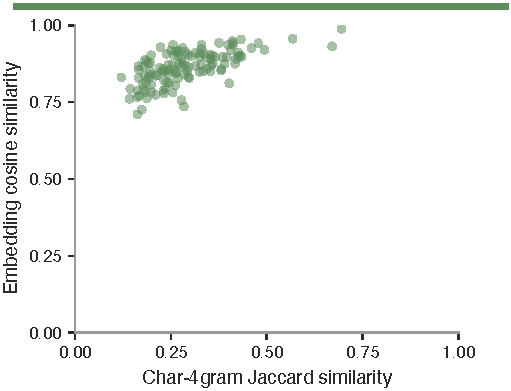
\includegraphics[width=.46\linewidth]{figures/out/emb_vs_lexical_both_correct.pdf}}
    &
    \subcaptionbox{\label{fig:emb-vs-lexical-f2i}}
      {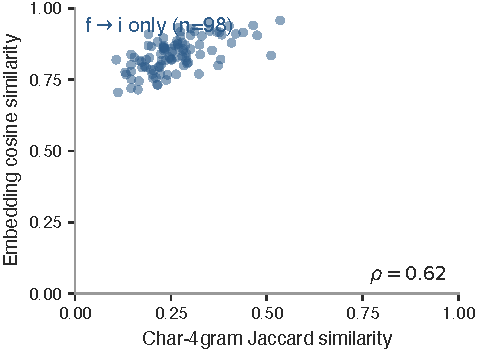
\includegraphics[width=.46\linewidth]{figures/out/emb_vs_lexical_f2i_only.pdf}} \\[3pt]
    \hline \\[-6pt]
    \subcaptionbox{\label{fig:emb-vs-lexical-i2f}}
      {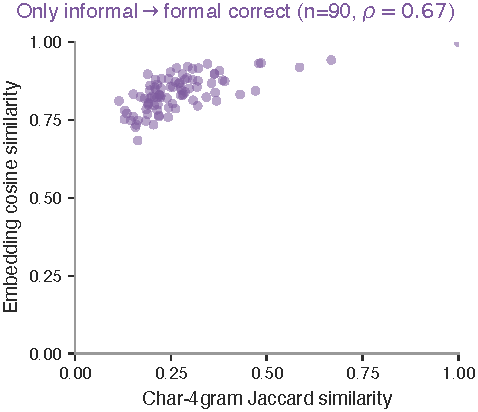
\includegraphics[width=.46\linewidth]{figures/out/emb_vs_lexical_i2f_only.pdf}}
    &
    \subcaptionbox{\label{fig:emb-vs-lexical-neither}}
      {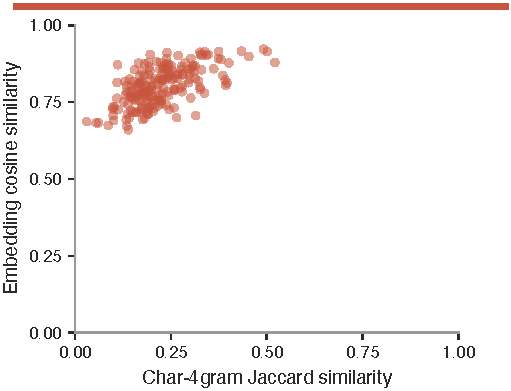
\includegraphics[width=.46\linewidth]{figures/out/emb_vs_lexical_neither.pdf}} \\
  \end{tabular}
  \arrayrulecolor{black}
  \caption{Embedding cosine vs.\ char-4gram Jaccard similarity for the
           500-pair f$\to$i rank-1 sample, split by direction-correctness
           bucket:
           \dotmark{groupGreen}~both directions rank-1 correct
              ($n{=}121,\ \rho{=}0.65$);
           \dotmark{groupBlue}~only f$\to$i correct
              ($n{=}98,\ \rho{=}0.62$);
           \dotmark{groupPurple}~only i$\to$f correct
              ($n{=}90,\ \rho{=}0.67$);
           \dotmark{groupRed}~neither direction correct
              ($n{=}191,\ \rho{=}0.60$).
           Spearman $\rho$ sits tightly around the overall 0.66 across all
           buckets; what shifts is the \emph{location} of the cloud, not
           its slope.}
  \label{fig:emb-vs-lexical}
\end{figure}
